%pictures and spectra
%tables and graphs
%statements of the result
% \begin{table*}
%     \caption{Characteristic \alpha line energy of several samples, listed with the bin of the MCA.}
%     \label{tab:bin-E}
%     \centering
%     \begin{tabular}{l S[table-format=3.0] S[table-format=3.3]}
%           \toprule
%           {Material} & {Bin} & {$E \: [\si{\kilo\eV}]$} \\
%           \midrule
%           {Cs} & 735 & 30.972 \\
%           {Ag} & 528 & 22.163  \\
%           \bottomrule
%     \end{tabular}
% \end{table*}

\section{Results}
\label{sec:Results}

In the following, the measurement results are going to be presented. 
Therefore some characterizations of the used lightsources are done, as well of other light sources, in order to understand their features as well as the impact of external noise.
 %LED emission spectra
\subsection{LED emission spectra}
\label{sec:LED}
\begin{figure*}
    \centering
\begin{subfigure}{.32\textwidth}
    \centering
    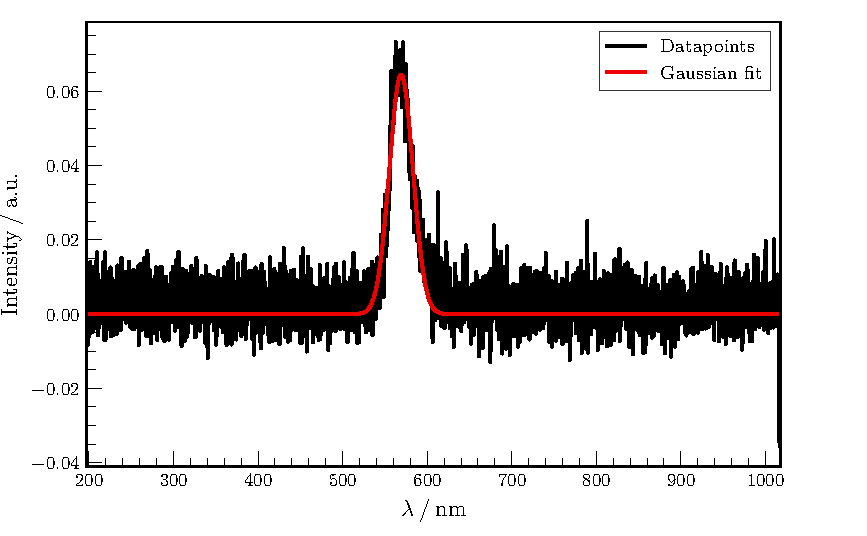
\includegraphics[width=\textwidth]{plots/LED-Green.pdf}
    \caption{Green LED lightsourse}
    \label{fig:LEDG}
\end{subfigure}
\begin{subfigure}{.32\textwidth}
    \centering
    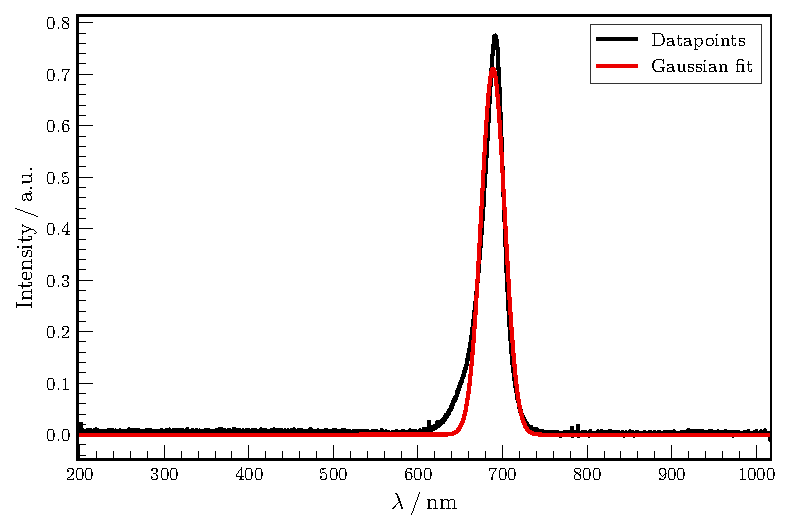
\includegraphics[width=\textwidth]{plots/LED-Red.pdf}
    \caption{Red LED lightsourse}
    \label{fig:LEDR}
\end{subfigure}
\begin{subfigure}{.32\textwidth}
    \centering
    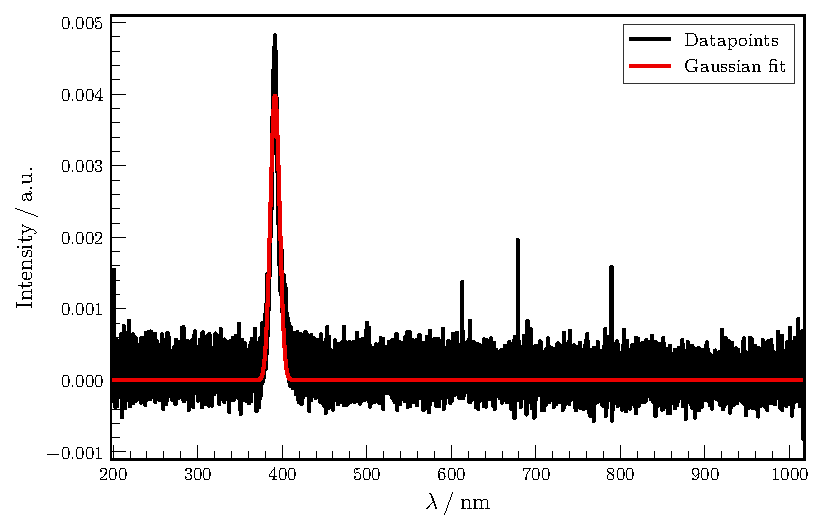
\includegraphics[width=\textwidth]{plots/LED-UV.pdf}
  \caption{UV LED lightsourse}
    \label{fig:LEDUV}
\end{subfigure}
\caption{Spectral measurement of different LED lightsourse. A Gaussian fit is implemented around the emmision peak.}
\end{figure*}


In figure \ref{fig:LEDG},\ref{fig:LEDR},\ref{fig:LEDUV} there are the spectra of a green, red and UV-LED, where a gaussian fit of the form 
\begin{equation}
    f(x,a,b,c) = a \times \exp{-\frac{(x-b)^2}{2 c^2}}
\end{equation}\label{eq:gauss}
has been introduced. Clearly a $\lambda_\text{peak}$ 
\begin{align*}
    \lambda_\text{peak,green} &= \SI{569.2 \pm 0.2}{\nano\meter} \\
    \lambda_\text{peak,red} &= \SI{688.68 \pm 0.05}{\nano\meter} \\
    \lambda_\text{peak,UV} &= \SI{391.5 \pm 0.1}{\nano\meter} \\
\end{align*}
can be found.

\subsection{Sample Spectra by UV-LED excitation}
\label{sec:samp_LED}

In the following the resulting spectra of the three unknown samples are presented, where the optical excitation is done by a UV-LED operated at a voltage of $\SI{2.98}{\volt}$.
The acquired data are averaged over 10 measurement cycles, and the integration time is $\SI{200}{\nano\second}$.
Also, a background correction has been done, where a spectrum, aquired without the sample is substracted from the luminescense spectrum.
The peak of the probe is still visible, as there is a scattering in the sample holder occuring.
By comparing the peaks in intensity but also in wavelength, it becomes clear that the probe is the more energetic, small wavelength and less intense one.


A gaussian fit \ref{eq:gauss} has been done for all three spectra, in order to obtain the peak wavelength of luminescence, as well as the spectral broadening, which corresponds to the variance, namely the parameter c of the fit.

% \begin{figure}
%     \captionsetup{width=0.9\linewidth}
%     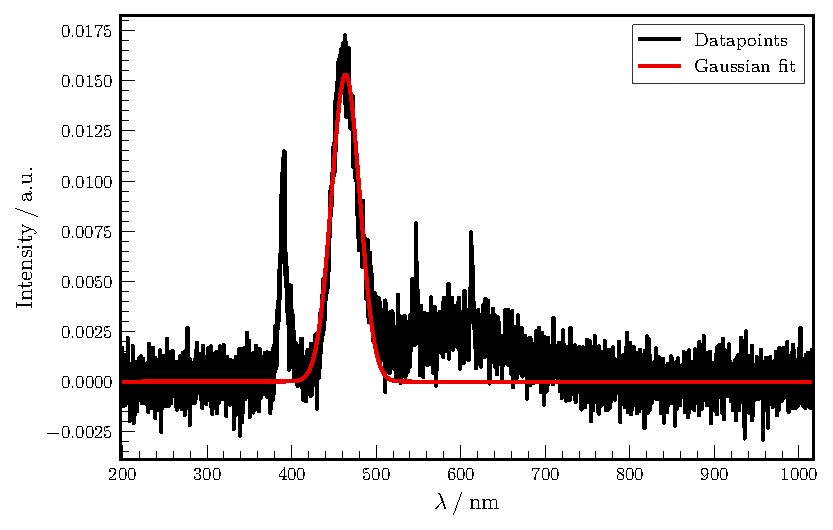
\includegraphics[width=0.5\textwidth]{plots/Samp_A_D.pdf}
%   \caption{Spectral measurement of sample A, excited by a UV-LED lightsource. A Gaussian fit of the peak contributed by luminescense is implemented.}
%     \label{fig:Samp_A_D}
% \end{figure}

% \begin{figure}
%     \captionsetup{width=0.9\linewidth}
%     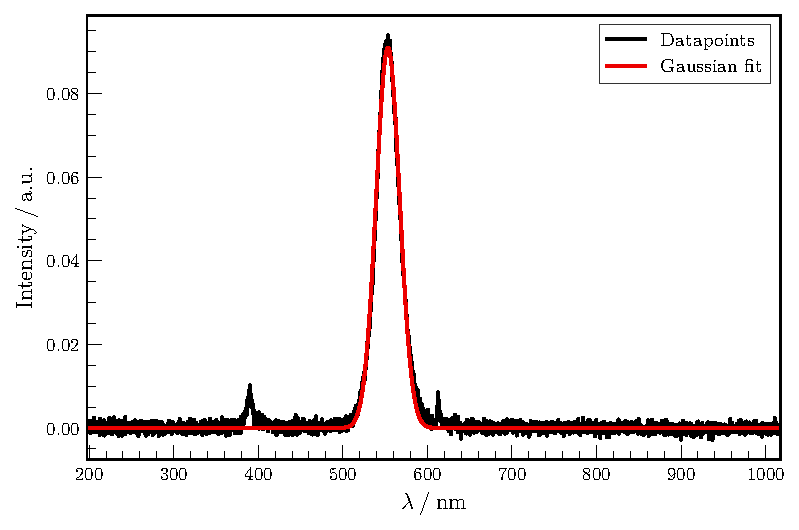
\includegraphics[width=0.5\textwidth]{plots/Samp_B_D.pdf}
%   \caption{Spectral measurement of sample B, excited by a UV-LED lightsource. A Gaussian fit of the peak contributed by luminescense is implemented.}
%     \label{fig:Samp_B_D}
% \end{figure}

% \begin{figure}
%     \captionsetup{width=0.9\linewidth}
%     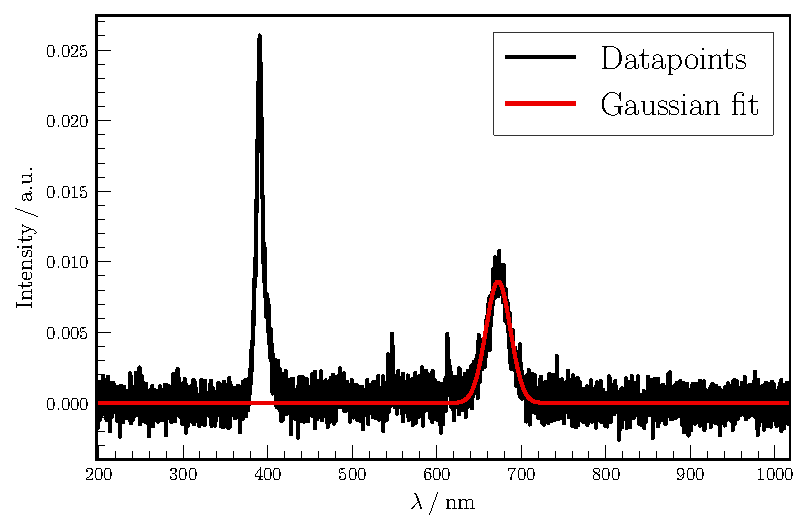
\includegraphics[width=0.5\textwidth]{plots/Samp_C_D.pdf}
%   \caption{Spectral measurement of sample C, excited by a UV-LED lightsource. A Gaussian fit of the peak contributed by luminescense is implemented.}
%     \label{fig:Samp_C_D}
% \end{figure}

%
\begin{figure*}
    \centering
\begin{subfigure}{.32\textwidth}
    \centering
    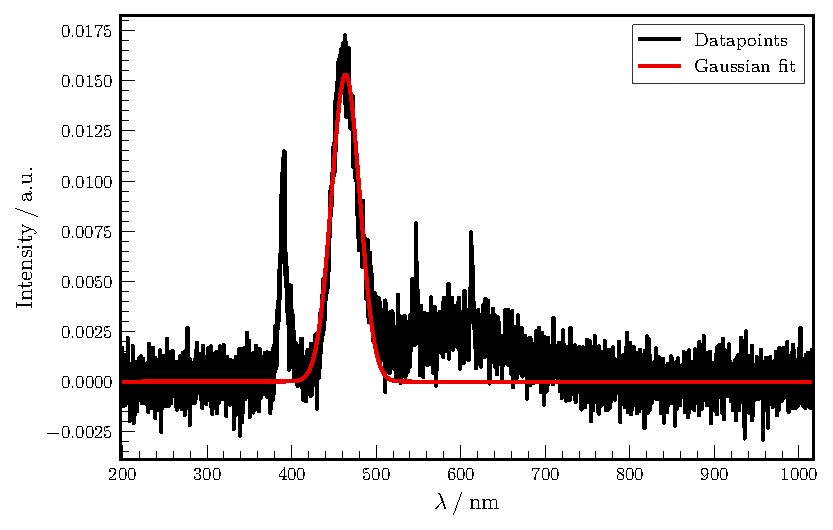
\includegraphics[width=\textwidth]{plots/Samp_A_D.pdf}
    \caption{Sample A spectrum}
    \label{fig:Samp_A_D}
\end{subfigure}
\begin{subfigure}{.32\textwidth}
    \centering
    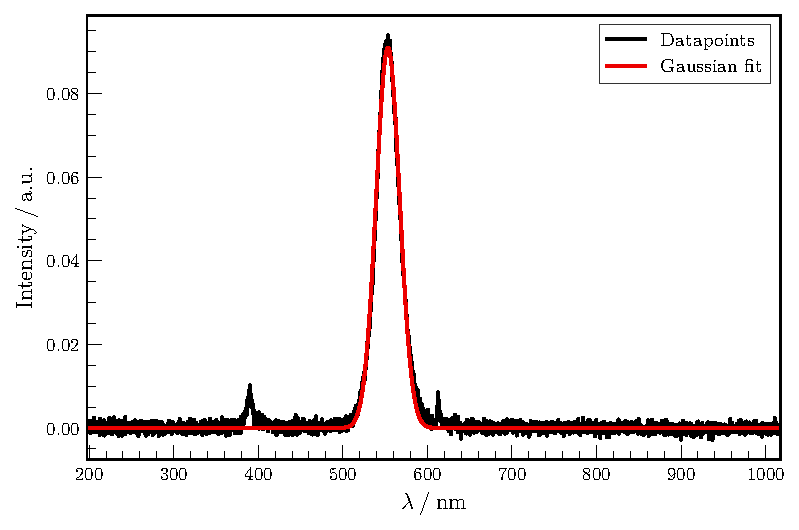
\includegraphics[width=\textwidth]{plots/Samp_B_D.pdf}
    \caption{Sample B spectrum}
    \label{fig:Samp_B_D}
\end{subfigure}
\begin{subfigure}{.32\textwidth}
    \centering
    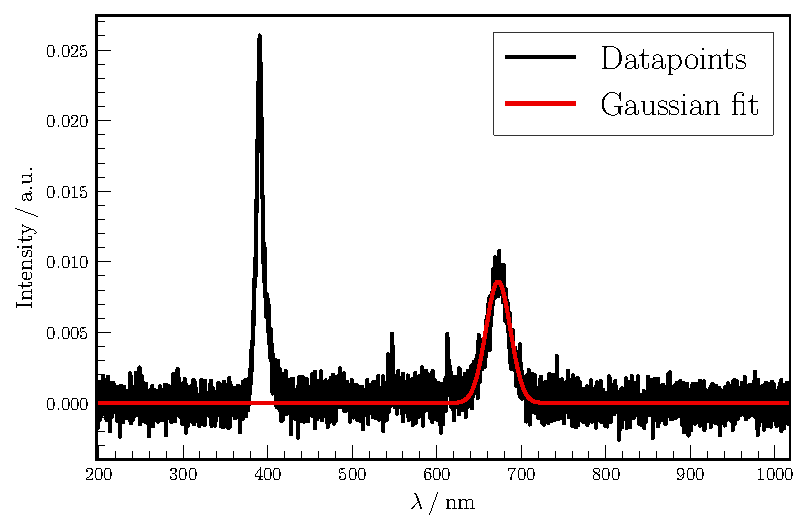
\includegraphics[width=\textwidth]{plots/Samp_C_D.pdf}
  \caption{Sample C spectrum}
    \label{fig:Samp_C_D}
\end{subfigure}
\caption{Spectral measurement of sample A,B and C, excited by a UV-LED lightsource. A Gaussian fit of the peak contributed by luminescense is implemented.}
\end{figure*}

The resulting peak wavelengths $\lambda_\text{peak}$ and spectral widening $\sigma$ are given in table \ref{tab:results-LED}.
% \begin{align*}
%     \lambda_\text{peak,A} &= \SI{463.9 \pm 0.2}{\nano\meter} \\
%     \sigma_\text{A} &= \SI{16.7 \pm 0.2}{\nano\meter} \\
%     \lambda_\text{peak,B} &= \SI{553.33 \pm 0.03}{\nano\meter} \\
%     \sigma_\text{B} &= \SI{13.93 \pm 0.03}{\nano\meter} \\
%     \lambda_\text{peak,C} &= \SI{672.6 \pm 0.5}{\nano\meter} \\
%     \sigma_\text{C} &= \SI{14.5 \pm 0.5}{\nano\meter}. \\
% \end{align*}
The wavelength, given in table \ref{tab:results-LED} is directly referred to the energy of the photon by equation \ref{eq:h}.
% \begin{align*}
%     E_\text{A} &= \SI{2.673 \pm 0.001}{\eV} \\
%     E_\text{B} &= \SI{2.241 \pm 0.001}{\eV} \\
%     E_\text{C} &= \SI{1.843 \pm 0.002}{\eV}. \\
% \end{align*}

Now, by assuming a diameter of $\SI{6}{\nano\meter}$ for the nanoparticles astimation of the nanoparticles is done.
There, the two equations \ref{eq:QD} and \ref{eq:E-G} are plugged into each other and solved for the concentration $x$, with the parapeters
\begin{align*}
    b          &= \SI{0.24}{\eV}\\
    E_g(CdS)   &= \SI{2.45}{\eV}\\
    E_g(CdSe)  &= \SI{1.74}{\eV}\\
    m^*_e(CdS) &= \num{0.21}\frac{1}{m_0}\\
    m^*_e(CdSe)&= \num{0.13}\frac{1}{m_0}\\
    m^*_h(CdS) &= \num{0.8}\frac{1}{m_0}\\
    m^*_h(CdS) &= \num{0.45}\frac{1}{m_0}.\\
\end{align*}\cite{instruction}

The resulting concentrations $x$ for the three samples are listed in table \ref{tab:results-LED}.
% \begin{align*}
%     x(sample A) &= \num{1.22}\\
%     x(sample B) &= \num{0.77}\\
%     x(sample C) &= \num{0.20}.\\
% \end{align*}

\begin{table*}
    \caption{Spectometral found peak wavelength $\lambda_\text{peak}$ and the standard derivation $\sigma$, as well as the calculated bandgap energy $E_g$ and sulfur concentration x. An UV LED is the excitation source.}
    \label{tab:results-LED}
    \centering
    \begin{tabular}{l S[table-format=3.2]@{${}\pm{}$}S[table-format=1.2] S[table-format=2.2]@{${}\pm{}$}S[table-format=1.2] S[table-format=1.3]@{${}\pm{}$}S[table-format=1.3] S[table-format=1.2]}
          \toprule
          {Sample} & \multicolumn{2}{c}{$\lambda \: [\si{\nano\meter}]$} & \multicolumn{2}{c}{$\sigma \: [\si{\nano\meter}]$} & \multicolumn{2}{c}{$E_g \: [\si{\eV}]$} & {Concentration} \\
          \midrule
          {A} & 463.9  & 0.2   & 16.7  & 0.2   & 2.673 & 0.001 & 1.22\\
          {B} & 553.33 & 0.03  & 13.93 & 0.03  & 2.241 & 0.001 & 0.77\\
          {C} & 672.6  & 0.5   & 14.5  & 0.5   & 1.843 & 0.002 & 0.20\\
          \bottomrule
    \end{tabular}
\end{table*}

The same procedure can be done for a probing UV laser. The spectra are depicted in figure \ref{fig:UV-sample-spectra}.
\begin{figure*}
    \centering
\begin{subfigure}{.32\textwidth}
    \centering
    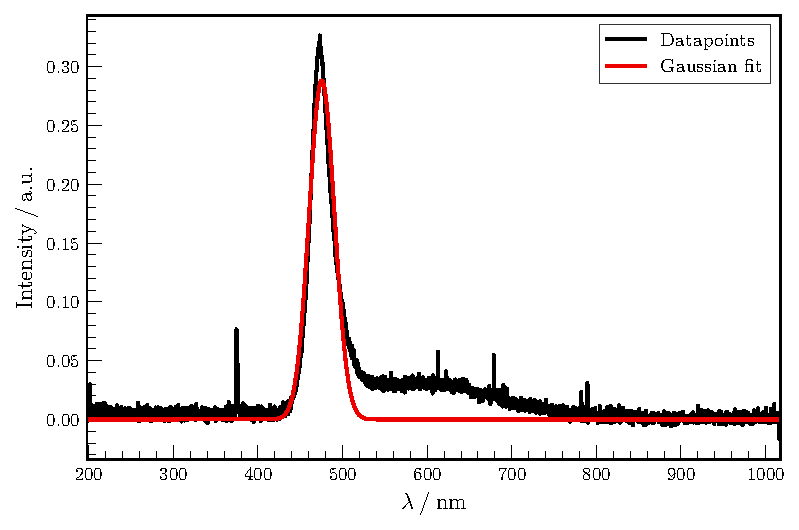
\includegraphics[width=\textwidth]{plots/Samp_A_D_UV.pdf}
    \caption{Sample A spectrum}
\end{subfigure}
\begin{subfigure}{.32\textwidth}
    \centering
    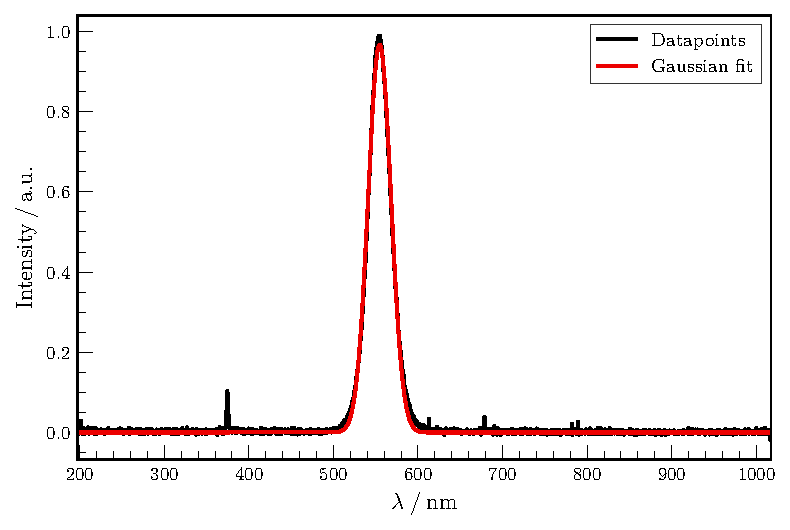
\includegraphics[width=\textwidth]{plots/Samp_B_D_UV.pdf}
    \caption{Sample B spectrum}
\end{subfigure}
\begin{subfigure}{.32\textwidth}
    \centering
    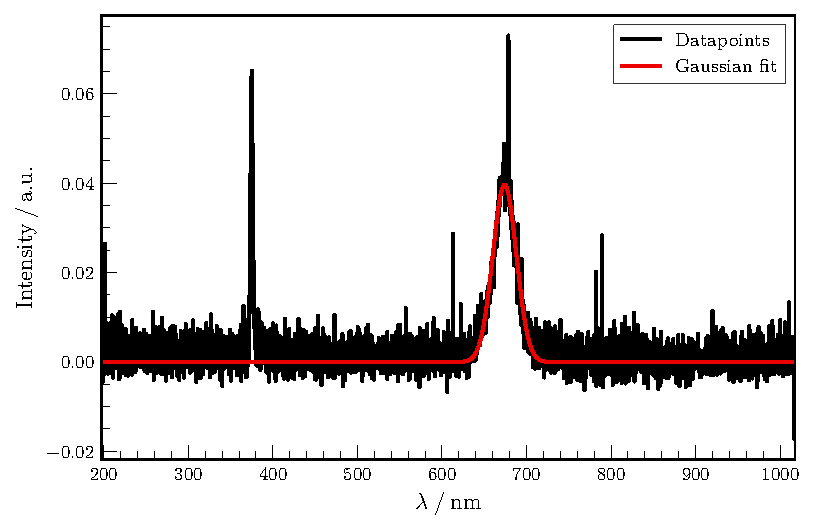
\includegraphics[width=\textwidth]{plots/Samp_C_D_UV.pdf}
  \caption{Sample C spectrum}
\end{subfigure}
\caption{Spectral measurement of sample A,B and C, excited by a UV-Laser lightsource. A Gaussian fit of the peak contributed by luminescense is implemented.}
\end{figure*}\label{fig:UV-sample-spectra}

The resulting emmision peak wavelengths, and thus the energies and material concentrations, calulated with the parameters given above, are summarized in table \ref{tab:results-Laser}. 
% \begin{align*}
%     \lambda_\text{peak,A} &= \SI{475.4 \pm 0.1}{\nano\meter} \\
%     \sigma_\text{A} &= \SI{15.0 \pm 0.1}{\nano\meter} \\
%     \lambda_\text{peak,B} &= \SI{554.58 \pm 0.02}{\nano\meter} \\
%     \sigma_\text{B} &= \SI{13.56 \pm 0.02}{\nano\meter} \\
%     \lambda_\text{peak,C} &= \SI{674.1 \pm 0.2}{\nano\meter} \\
%     \sigma_\text{C} &= \SI{14.0 \pm 0.2}{\nano\meter}, \\
% \end{align*}
% and thus the energies are
% \begin{align*}
%     E_\text{A} &= \SI{2.608 \pm 0.001}{\eV} \\
%     E_\text{B} &= \SI{2.236 \pm 0.000}{\eV} \\
%     E_\text{C} &= \SI{1.840 \pm 0.001}{\eV}. \\
% \end{align*}
% Using the same parameters as above, one comes to the concentrations of
% \begin{align*}
%     x(sample A) &= \num{1.16}\\
%     x(sample B) &= \num{0.77}\\
%     x(sample C) &= \num{0.19}.\\
% \end{align*}

\begin{table*}
    \caption{Spectometral found peak wavelength $\lambda_\text{peak}$ and the standard derivation $\sigma$, as well as the calculated bandgap energy $E_g$ and sulfur concentration x. An UV Laser is the excitation source.}
    \label{tab:results-Laser}
    \centering
    \begin{tabular}{l S[table-format=3.2]@{${}\pm{}$}S[table-format=1.2] S[table-format=2.2]@{${}\pm{}$}S[table-format=1.2] S[table-format=1.3]@{${}\pm{}$}S[table-format=1.3] S[table-format=1.2]}
          \toprule
          {Sample} & \multicolumn{2}{c}{$\lambda \: [\si{\nano\meter}]$} & \multicolumn{2}{c}{$\sigma \: [\si{\nano\meter}]$} & \multicolumn{2}{c}{$E_g \: [\si{\eV}]$} & {Concentration} \\
          \midrule
          {A} & 475.4  & 0.1   & 15.0  & 0.1   & 2.608 & 0.001 & 1.16\\
          {B} & 554.58 & 0.02  & 13.56 & 0.02  & 2.236 & 0.000 & 0.77\\
          {C} & 674.1  & 0.2   & 14.0  & 0.2   & 1.843 & 0.001 & 0.19\\
          \bottomrule
    \end{tabular}
\end{table*}

\subsection{Perovskite}
\label{sec:perovsikite-measure}

For a LED probe there could not be measured a emission spectrum for the perovskite sample. Thus, the UV-laser is used and the measured spectrum is given in figure \ref{fig:perov}.
\begin{figure}
    \captionsetup{width=0.9\linewidth}
    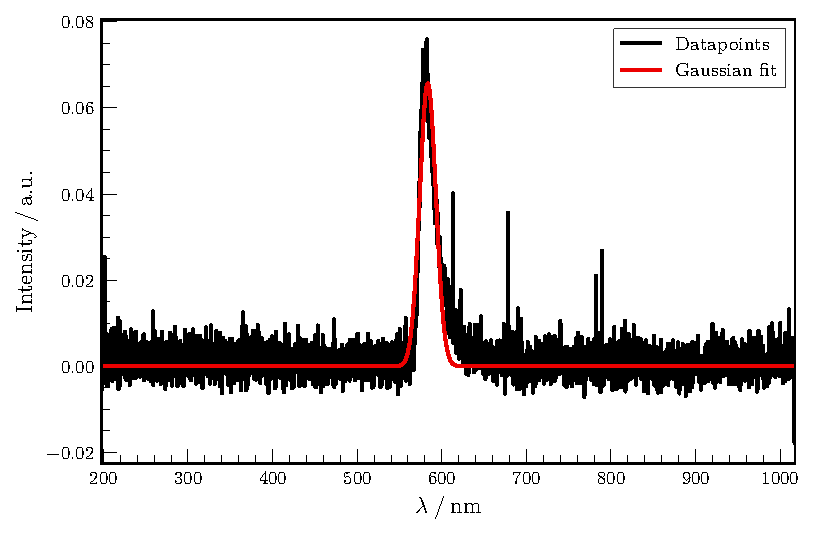
\includegraphics[width=0.5\textwidth]{plots/Samp_P_UV.pdf}
  \caption{Spectral measurement of the perovskite sample, excited by a UV-Laser lightsource. A Gaussian fit of the peak contributed by luminescense is implemented.}
    \label{fig:perov}
\end{figure}
The peak wavelength is $\lambda_\text{peak}= \SI{583.5 \pm 0.1}{\nano\meter}$, which gives directly a bandgap of 
$E_\text{Perovskite} = \SI{2.13}{\eV}$.

